\input{SlideInclude.tex}

\title[Ideas]{The Economics of Ideas}


\begin{document}
\maketitle

\section{Definition}
\begin{frame}{Ideas}
We use the term ``idea'' to refer to any
\begin{itemize}
	\item .. plan, blueprint, recipe, design, or business idea
	\item .. that tells us how to combine factors of production (labor, capital)
	\item .. to produce some product that someone might be willing to pay for
\end{itemize}
Ideas are not just about ``technology'':
\begin{itemize}
	\item The latest iteration of ChatGPT is an idea, yes
	\item ..but so is identifying a good place to locate a Starbucks
	\item ..and so is a restaurant concept that attracts patrons
\end{itemize} 
\end{frame}

\section{Measurement}
\begin{frame}{Measuring ideas}
It's hard to measure this. \textit{One} way is to look at formal applications for ideas, patents.
\begin{itemize}
	\item Patents tend to skew towards technological ideas
	\item Patents do not cover all ideas (think of the Starbucks, or the recipe for Coke)
	\item Each patent is not equal. Some are dumb, some are transformative.
\end{itemize}
\end{frame}

\begin{frame}{Patent data in the United States}
Patents Issued in the United States, by Country of Origin
\begin{center}
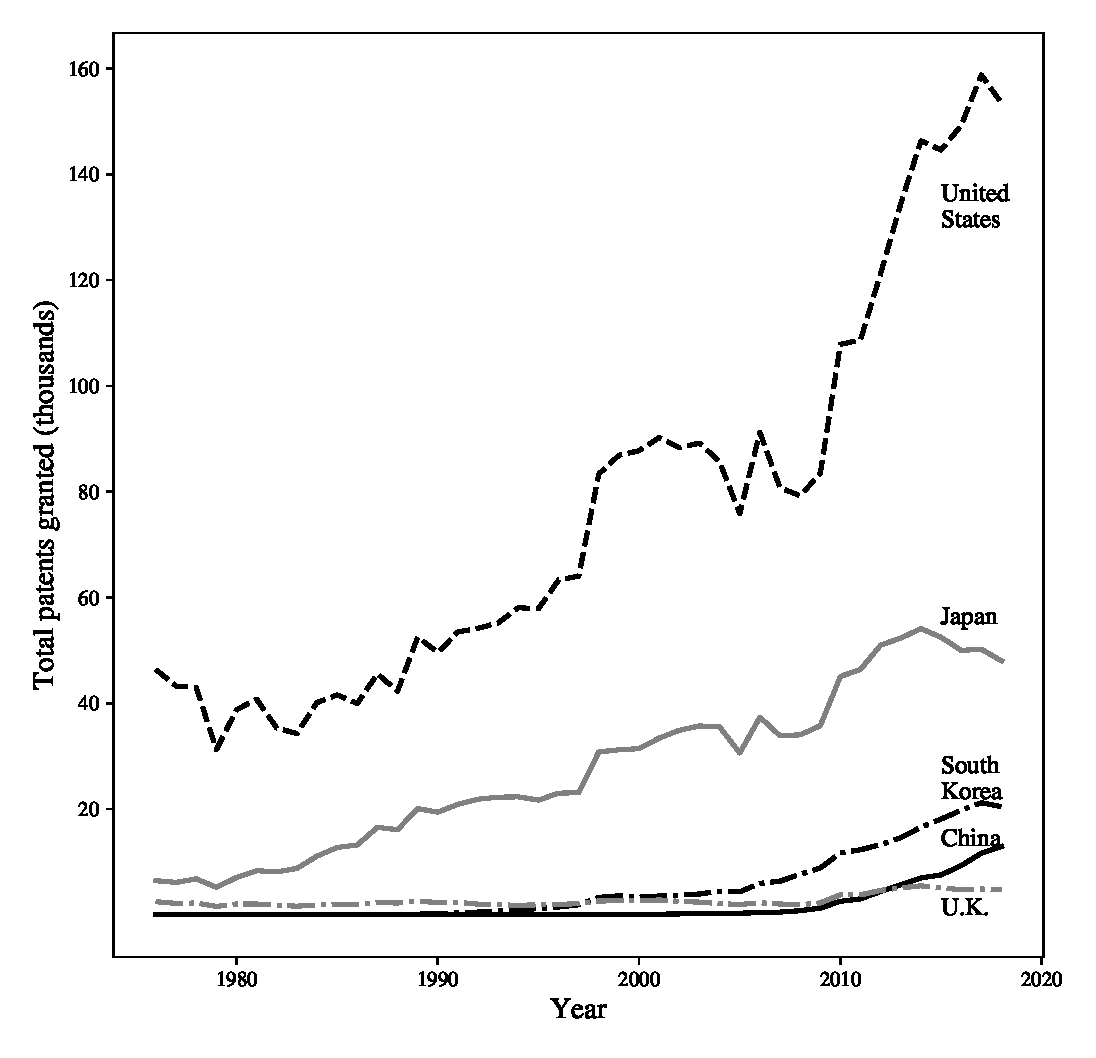
\includegraphics[height = 3in]{../Figures/fig-ch4-fig1.eps}
\end{center}
\end{frame}

\begin{frame}{Measuring effort}
A crucial concept is that creating ideas takes effort. 
\begin{itemize}
	\item Mainly time. Possibly capital in terms of labs, computers, etc. 
	\item We typically call this effort R\&D
	\item R\&D uses productive labor and capital firms and individuals are making a deliberate choice to do this versus something else
	\item Ultimately the process of growth depends on this choice
\end{itemize}
\end{frame}

\begin{frame}{R\&D effort}
Number of R\&D Workers (FTE), by Country
\begin{center}
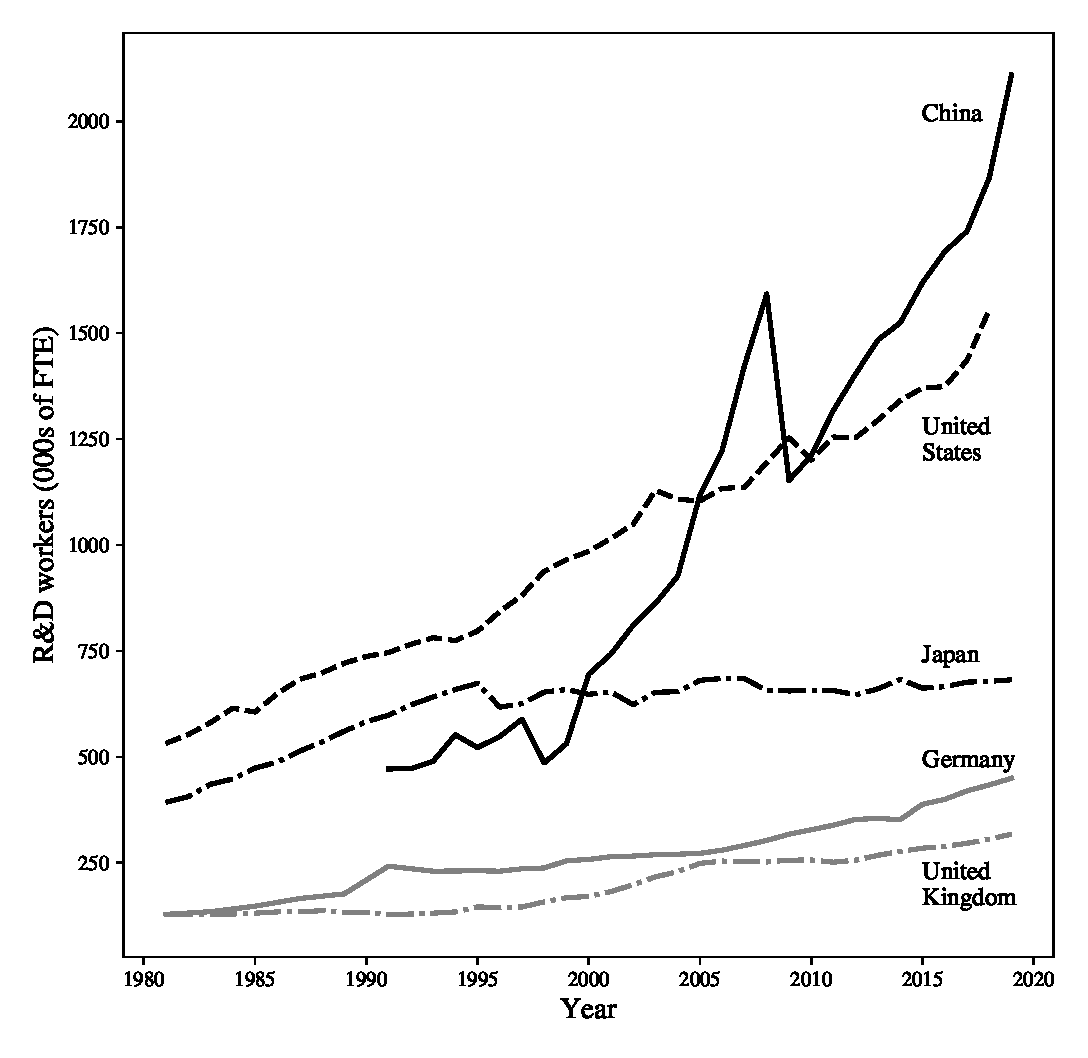
\includegraphics[height = 3in]{../Figures/fig-ch4-fig2.eps}
\end{center}
\end{frame}

\begin{frame}{R\&D effort}
R\&D Workers as a Percent of Employment, by Country
\begin{center}
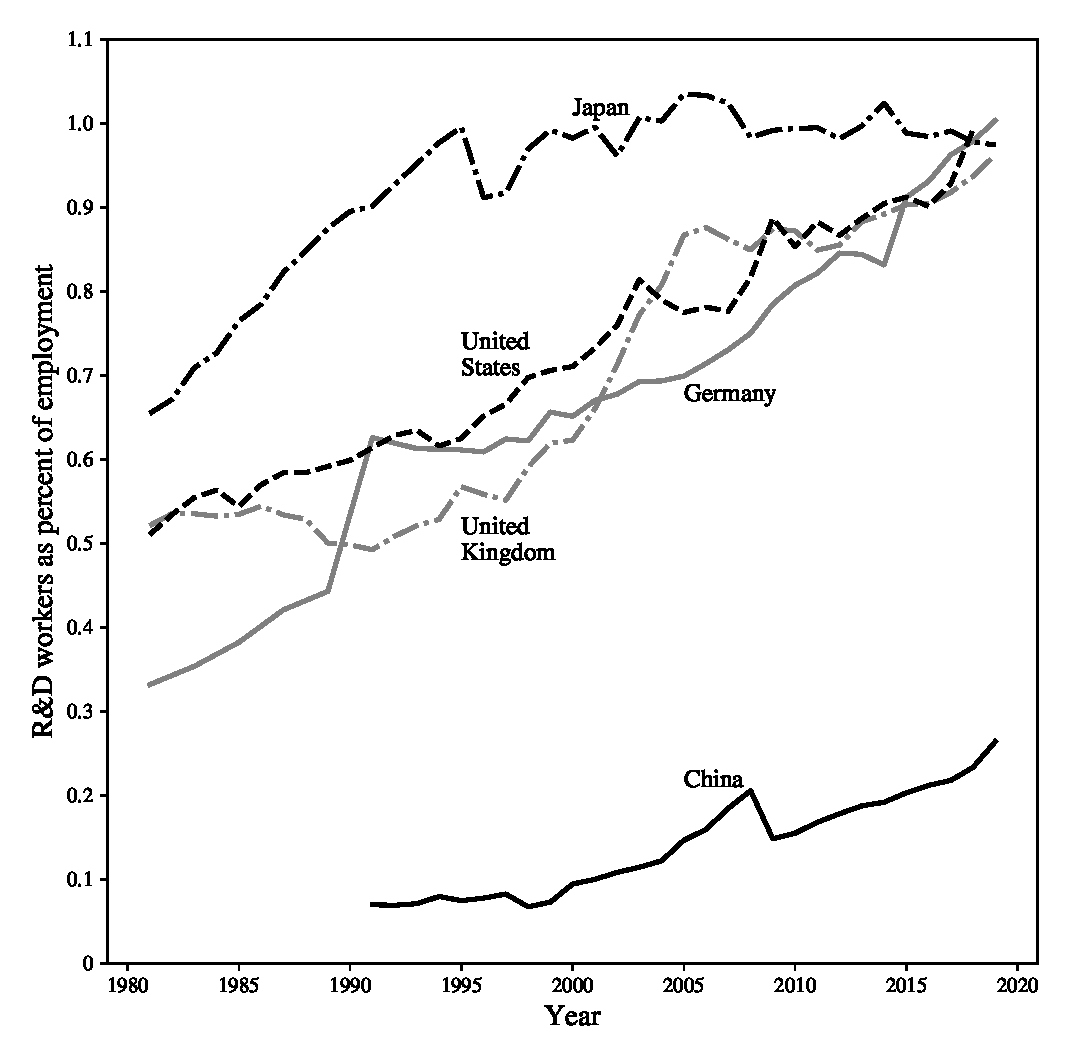
\includegraphics[height = 3in]{../Figures/fig-ch4-fig3.eps}
\end{center}
\end{frame}

\section{Economics}

\begin{frame}{Non-rivalry}
The key quality of ideas for growth is that they are \textbf{non-rival}.
\begin{itemize}
	\item One person using the idea does not prevent someone else from using it
	\item They can be copied/used with zero or close to zero cost
\end{itemize}
Contrast this to things like labor and capital which are \textbf{rival}.
\begin{itemize}
	\item If you use a rival good, I cannot
	\item It takes time and/or resources to copy a rival input
\end{itemize}
\end{frame}

\begin{frame}{Why do R\&D?}
Economies are putting more effort into R\&D. Why?
\begin{itemize}
	\item Ideas are non-rival but it takes time/effort to create them \textit{once}
	\item Once created the idea can be reused without diminishing it
	\item Production using an idea is increasing returns
	\item ..meaning high fixed costs and low/zero marginal cost
\end{itemize}
\end{frame}

\begin{frame}{Intuition of increasing returns}
Think about a simple structure for possible innovators
\begin{itemize}
	\item Someone can pay a fixed cost, $F$, to create an idea.
	\item With that idea they can earn operating profits $V = pY - cY$
	\item It only makes sense to innovate and operate if $V \geq F$
\end{itemize}
What does this imply about what price, $p$, you have to charge?
\end{frame}

\begin{frame}{Increasing returns}
Costs Functions with Increasing Returns
\begin{center}
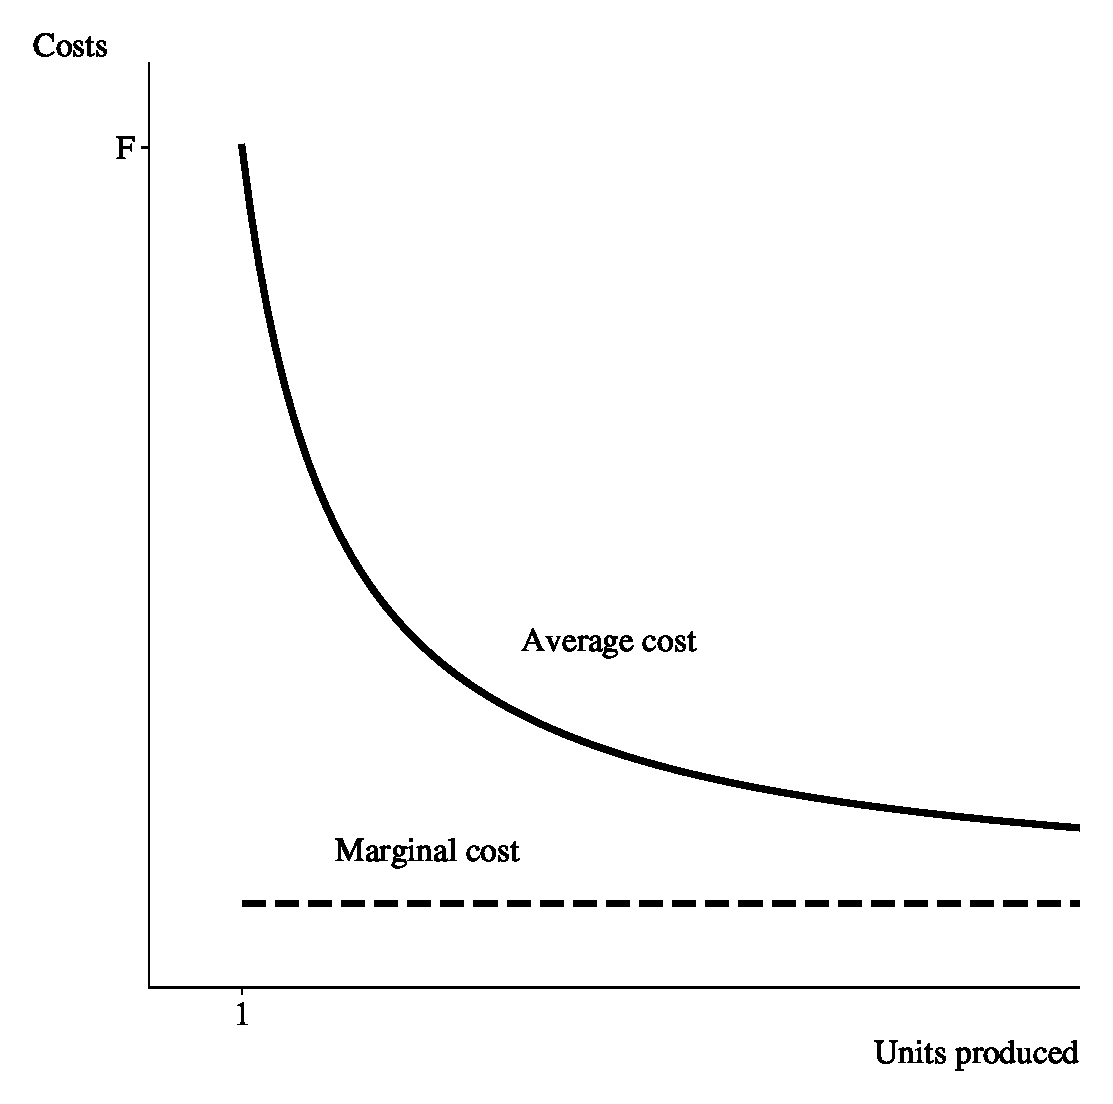
\includegraphics[height = 3in]{../Figures/fig-ch4-fig5.eps}
\end{center}
\end{frame}

\begin{frame}{Imperfect competition}
The only way someone will innovate and operate is if $p > c$
\begin{itemize}
	\item Competitive markets (allowing entry of copies) will drive $p = c$
	\item Competitive markets maximize output of existing products, but $p < AC$ and profits are negative
	\item Innovation requires $p > c$ which implies \textit{imperfect competition}
	\item Innovators need to market power to ensure $V \geq F$
\end{itemize}
\end{frame}

\begin{frame}{Excludability}
\textbf{Excludability} is what allows you to stop someone from using or copying your product or idea
\begin{itemize}
	\item Excludability is closely related to property rights
	\item Excludability is almost always created by policy/law, not inherent
	\item Titles, patents, copyrights, etc. are ways to create excludability
	\item Excludability means other people need to pay for your non-rival idea
\end{itemize}
\end{frame}

\section{Scale}
\begin{frame}{The importance of scale}
Why does Houston (7 mil metro area) have better food than Tulsa (1 mil metro area)?
\begin{itemize}
	\item There are more potential restauranteurs with more varied backgrounds. There are more novel ideas to try (e.g. a Nigerian/Mexican fusion food truck)
	\item There are more potential customers with more varied tastes. Weird niche ideas can thrive (e.g. \textit{someone} will love Nigerian/Mexican food)
\end{itemize}
\end{frame}

\begin{frame}{Scale and rivalry}
Think about rival inputs like capital or natural resources:
\begin{itemize}
	\item More people allows us to make (or mine or extract) more of the input
	\item The amount of input \textit{per capita} goes down with more people
	\item There is a race between production and dilution of rival inputs
\end{itemize}
With non-rival inputs like ideas:
\begin{itemize}
	\item More people still allow us to make more of the input
	\item But the per capita stock of ideas per capita \textit{does not go down}
	\item There is no ``race'' between R\&D and dilution of non-rival ideas
\end{itemize}
\end{frame}

\begin{frame}{Ideas and scale}
Take non-rivalry of ideas seriously:
\begin{itemize}
	\item More people means more ideas
	\item More ideas means higher GDP per capita
	\item GDP per capita is \textit{positively} related to the size of population/market
	\item Growth rate of GDP per capita is \textit{positively} related to growth rate of population
\end{itemize}
\end{frame}

\begin{frame}{Population and living standards}
World Population and GDP per capita, 1820-2019
\begin{center}
\includegraphics[height = 3in]{../Figures/fig-ch4-fig6.eps}
\end{center}
\end{frame}

\begin{frame}{Population and living standards}
Growth Rate of World Population and GDP per capita, 1820-2019
\begin{center}
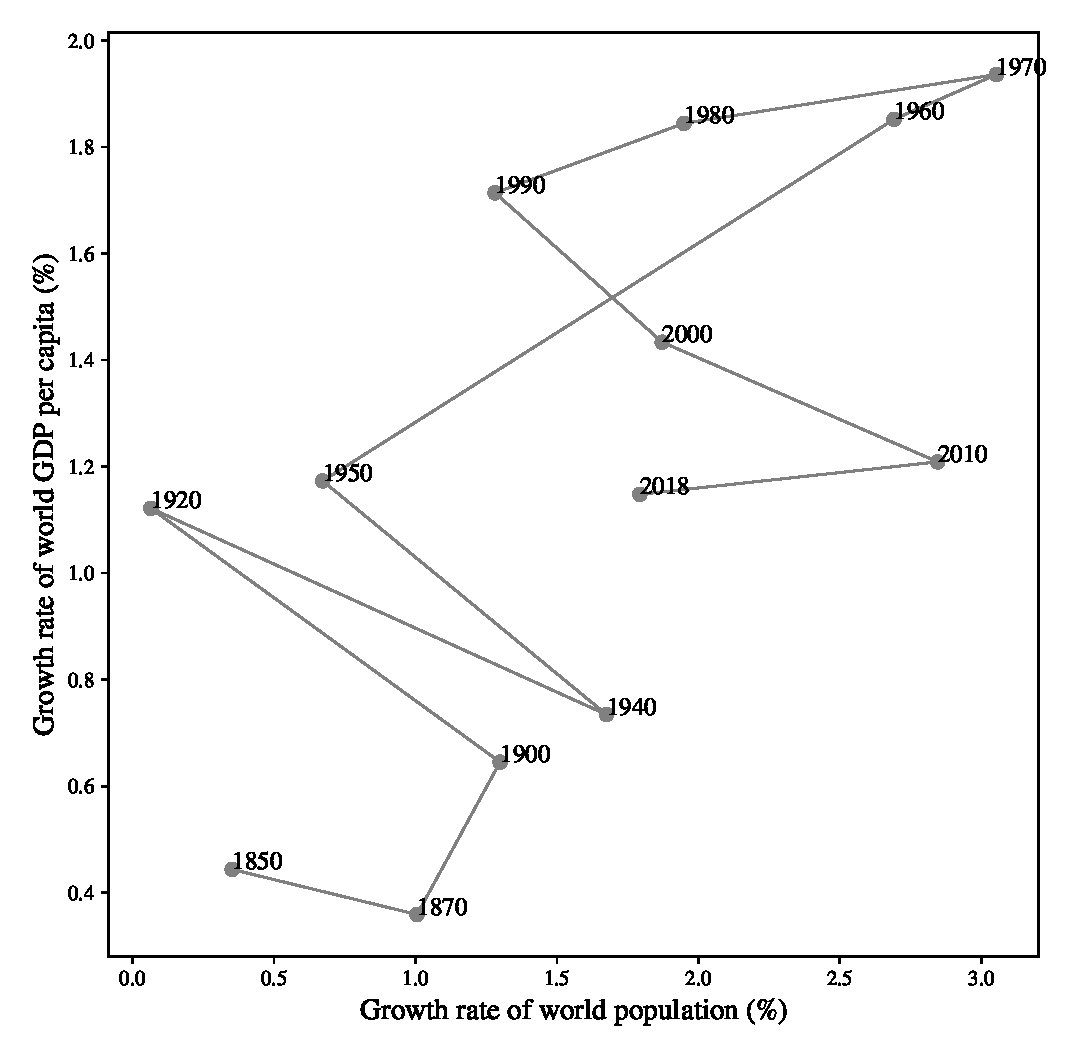
\includegraphics[height = 3in]{../Figures/fig-ch4-fig7.eps}
\end{center}
\end{frame}

\begin{frame}{Market size}
Population/market size matters for implementing ideas:
\begin{itemize}
	\item Assume entry makes $F \approx V$, so $F \approx (p-c)Y$:
	\item The bigger population the more units you can sell, $Y$, 
	\item This allows for either a smaller $p-c$ markup
	\item ..or for a given $p-c$ markup a bigger $F$ can be supported
\end{itemize}
Bigger markets allow for either lower markups (low $p-c$) or ``harder'' ideas (higher $F$)
\end{frame}

\end{document}